\vspace{-0.3cm}
Depois de uma viagem para lá de conturbada, finalmente as equipes
chegaram no local da Maratona de Programação deste ano. Ao
chegar, se depararam com um problema:
as máquinas, rodando nas problemáticas JVMs (\textit{Java Virtual Machine}),
estão travando demais.

Inicialmente, as equipes estão posicionadas em círculo, da equipe 1 à equipe
$N$, em sentido horário, e a equipe $i$ está utilizando a máquina $i$.
Quando acontece algum problema com as JVMs, a organização reinicia as máquinas e faz
um rodízio, no qual a máquina que cada equipe está usando
passa para a equipe que está a sua esquerda no círculo.

Cansadas, algumas equipes estão desistindo da competição e
indo embora. Quando uma equipe desiste, a máquina que ela estava utilizando é
descartada. Como exemplo, a figura abaixo apresenta: A) a posição inicial de
$N=4$ equipes e suas máquinas; B) o rodízio de máquinas após um problema; C) a
equipe 3 desistiu; D) o rodízio após outro problema.

\vspace{-0.4cm}
\begin{center}
    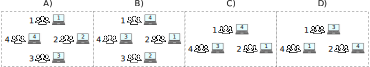
\includegraphics[scale=0.45]{rage/rage.png}
\end{center}

\vspace{-0.4cm}
Dada a sequência de problemas e de desistências que ocorreram, determine quais equipes
sobraram e com quais máquinas elas ficaram ao final da prova.

\subsection*{Entrada}

A primeira linha contém dois inteiros $N$ e $M$
($1 \leq N, M \leq 10^5$), o número de equipes e de acontecimentos,
respectivamente. A próxima linha contém $M$ inteiros $A_i$ indicando os
acontecimentos, na ordem em que aconteceram. $A_i=0$ indica um problema ocorrido
e um rodizio feito, enquanto $1 \leq A_i \leq N$ indica a desistência da equipe
$A_i$. Sobrará no mínimo uma equipe ao final da competição, e
nenhuma equipe desiste mais de uma vez.

\subsection*{Saída}

Para cada equipe que sobrou, imprima uma linha
com $i$ $c$ , indicando que a equipe $i$ ficou com a máquina $c$ no
final da prova.
Imprima em ordem crescente dos números das equipes.

\vspace{-0.3cm}
\begin{table}[!h]
\centering
\begin{tabular}{|l|l|}
\hline
\begin{minipage}[t]{3in}
\textbf{Exemplo de entrada}
\begin{verbatim}
4 3
0 3 0
\end{verbatim}
\vspace{1mm}
\end{minipage}
&
\begin{minipage}[t]{3in}
\textbf{Exemplo de saída}
\begin{verbatim}
1 3
2 4
4 1
\end{verbatim}
\vspace{1mm}
\end{minipage} \\
\hline
\end{tabular}
\end{table}

\vspace{-0.3cm}
\begin{table}[!h]
\centering
\begin{tabular}{|l|l|}
\hline
\begin{minipage}[t]{3in}
\textbf{Exemplo de entrada}
\begin{verbatim}
3 3
0 0 1
\end{verbatim}
\vspace{1mm}
\end{minipage}
&
\begin{minipage}[t]{3in}
\textbf{Exemplo de saída}
\begin{verbatim}
2 3
3 1
\end{verbatim}
\vspace{1mm}
\end{minipage} \\
\hline
\end{tabular}
\end{table}
